\lettrine{I}{n} questo capitolo si andranno a mostrare i protocolli usati per l'implementazione delle operazioni compiute dall'entità di rete. Si farà inoltre uso di \textit{sequence diagram} per i protocolli più articolati.

\section{Protocolli Server}
Il server come descritto precedentemente si occupa di eseguire le tre operazioni descritte precedentemente per la gestione della lista dei peer. Per questo motivo esso è stato implementato come semplice server iterativo, implementazione che, unita al basso tasso di richieste da servire e al meccanismo di autorizzazione di seguito descritto, evita inutile spreco di risorse.

\subsection{Protocollo d'autenticazione}
Il protocollo d'autenticazione viene eseguito sia dai peer che dai wallet che effetuano una richiesta di aggancio alla rete al server.\\ Tale protocollo prevede l'invio della password \footnote{la password viene scelta in fase di lancio del server passandola con l'apposita opzione da riga di comando. In caso di omissione, la password di default utilizzata è "VitCoin".} di rete inviata sotto forma di hash da parte del client. Se la password è corretta, il server invierà una conferma e si metterà in attesa della macro corrispondete ad una delle operazioni che è in grado di svolgere. Altrimenti comunicherà al client che la password è sbagliata è si metterà in attesa di nuove richieste di autenticazione.

\subsection{Protocollo d'aggancio peer}
\begin{figure}[H]
  \centering
  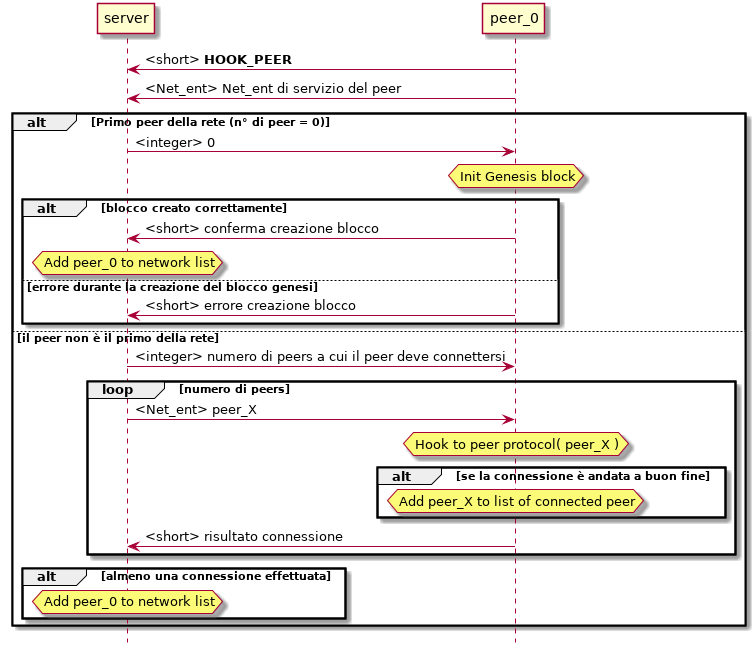
\includegraphics[scale=0.50]{hookpeer.png}    
  \caption{aggancio di un peer alla rete}
  \label{fig:hook_peer}
\end{figure}

La figura \ref{fig:hook_peer} mostra il protocollo che scatta con l'invio della apposita macro\footnote{HOOK\_PEER}, subito dopo l'autenticazione andata a buon fine da parte del peer. \\Il protocollo inizia con il peer che invia la propria Net\_ent di servizio al server. Da qui in poi le casistiche possibili sono 2:

\begin{enumerate}
\item il peer che si sta agganciando alla rete \textit{è il primo}. \\Ciò comporta che il server si mette in attesa della conferma di avvenuta crazione del blocco genesi da parte del peer. In caso di esito positivo il server lo aggiunge alla rete.
\item il peer che si sta agganciando alla rete \textit{non è il primo}. \\ In questo caso il server invia il numero minimo di peers con cui il nuovo peer deve provare la connessione. Successivamente invia uno alla volta le Net\_ent di servizio dei peer e conta il numero di connessioni riuscite al nuovo peer. Se almeno una connessione è riuscita, il nuovo peer viene aggiunto alla rete.
\end{enumerate}

\subsection{Protocollo d'aggancio wallet}
Il protocollo d'aggancio di un wallet alla rete è molto più semplice di quello utilizzato dai peer.\\ Infatti esso si compone al più di sue sole comunicazioni.
Dopo la corretta autenticazione e l'invio della macro  corrispondente da parte del wallet\footnote{HOOK\_WALLET}, il server gli invia sotto forma di intero il numero di peer attualmente presenti nella rete. Se tale numero è maggiore di 0 allora il server sceglie un peer a caso e ne invia la Net\_ent di servizio al wallet.

\subsection{Protocollo di chiusura peer}
Protocollo ancora più semplice che prevede che, un peer facente parte della rete che sta per spegnersi (dopo essersi autenticato ed aver inviato l'apposita macro\footnote{CLOSE\_PEER}) invii la propria Net\_ent di servizio al server, il quale la estrarrà dalla lista di Net\_ent rappresentante la rete.

\section{Protocolli Peer}
Come detto precedentemente un peer si occupa sostanzialmente di 3 macro compiti riguardanti rispettivamente: la gestione delle connessioni con gli altri peer e i wallet; l'aggiornamento della sua copia della blockchain con diffusione dei blocchi creati;  servire le richieste dei wallet.\\
L'aggancio alla rete del peer è stato spiegato nella parte che riguarda l'interazione con il server nella sezione precedente. 
In questa sezione saranno spiegati i protocolli che prevedono la comunicazione fra peer riguardanti la gestione delle connessioni e la trasmissione di blocchi.\\
I protocolli riguardanti le comunicazioni fra peer e wallet saranno invece spiegati nella sezione riguardante quest'ultimi.

\subsection{Protocollo d'aggancio ad un peer}
\begin{figure}[H]
  \centering
  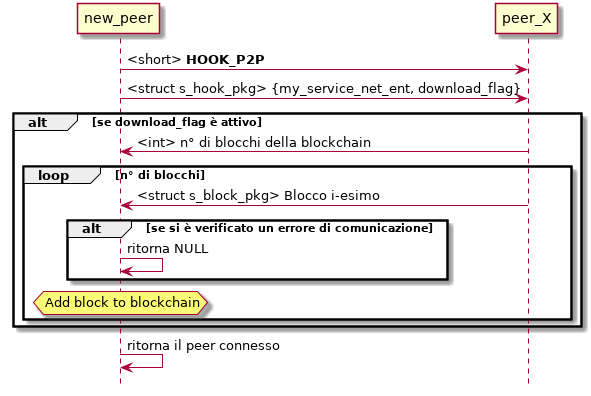
\includegraphics[scale=0.50]{hookp2p.png}    
  \caption{aggancio di un peer ad un altro peer}
  \label{fig:hook_p2p}
\end{figure}
In figura \ref{fig:hook_p2p} è mostrato il sequence diagram che spiega la funzione si permette ad un nuovo peer di agganciarsi ad un peer già agganciato alla rete. \\ Dopo l'apposita macro\footnote{HOOK\_P2P}, il nuovo peer invia un pacchetto contenente la propria Net\_ent di servizio e un flag passato come parametro, il quale indica se il nuovo blocco desidera oppure no scaricare la blockchain. \\L'utilità di tale flag sta nel fatto che un nuovo peer che si aggancia alla rete, si aggancia al numero di peer indicatogli dal server. Tuttavia risulta necessario effettuare il download della blockchain solo dal primo peer, il quale, a sua volta, (una volta che il nuovo peer avrà terminato la connessione alla rete e sarà pronto a ricevere  blocchi) provvederà a passargli i nuovi blocchi che sono stati creati mentre l'aggancio veniva ultimato.

\subsection{Protocolli di trasmissione/ricezione blocchi}
\begin{figure}[H]
  \centering
  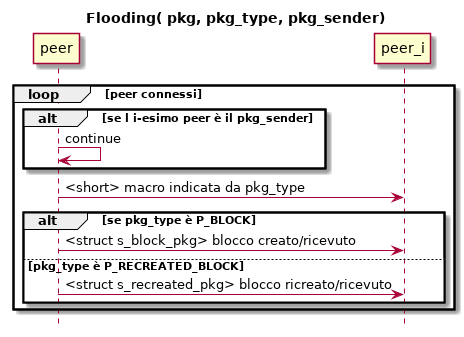
\includegraphics[scale=0.50]{flooding.png}    
  \caption{diffusione di un blocco}
  \label{fig:flooding}
\end{figure}

Come mostrato in figura \ref{fig:flooding} il protocollo di trasmissione\footnote{chiamato flooding(inondazione)  per il modo in cui viene trasmesso il blocco e cioè "inondando" i peer connessi.} è lo stesso indipendente dal tipo di blocco che si vuole trasmettere grazie all'utilizzo di un apposito flag. Viene inoltre passato come parametro la Net\_ent del peer che sta \textit{sta inviando}\footnote{il peer che \textit{invia} potrebbe essere sia il peer che sta eseguendo la funzione di flooding(cioè il creatore del blocco), sia uno dei peer connessi che ovviamente non ha bisogno di ricevere il blocco che lui stesso ci ha inviato (blocco ricevuto da altri).} il pacchetto in modo da evitare dei loop dei blocchi sulla rete.

\section{Protocolli Wallet}
In questa sezione saranno mostrati i protocolli adottati per la comunicazione del wallet con il peer a cui esso è agganciato.\\ Non si riporta la procedura d'aggancio, la quale consiste sostanzialmente solo dell'invio della apposita macro \footnote{HOOK\_W2P}, seguita dall'invio della propria Net\_ent del wallet e dalla conferma di ricezione inviata dal peer.

\subsection{Protocollo per nuova transazione}
\begin{figure}[H]
  \centering
  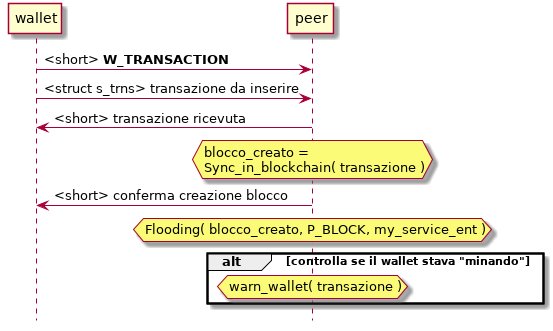
\includegraphics[scale=0.40]{w_transaction.png}    
  \caption{richiesta di una nuova transazione}
  \label{fig:w_transaction}
\end{figure}

Il protocollo utilizzato per la creazione di una nuova transazione viene usato sia nel caso di scambio di \vitcoin verso altri wallet che per il "mining"\footnote{ovviamente la procedura di mining sarà soltanto simulata, e serve sostanzialmente solo per permettere al wallet di acquisire \vitcoin come ricompensa appunto per il "mining" effettuato} di nuovi \vitcoin.

\subsection{Protocollo di richiesta saldo}
\begin{figure}[H]
  \centering
  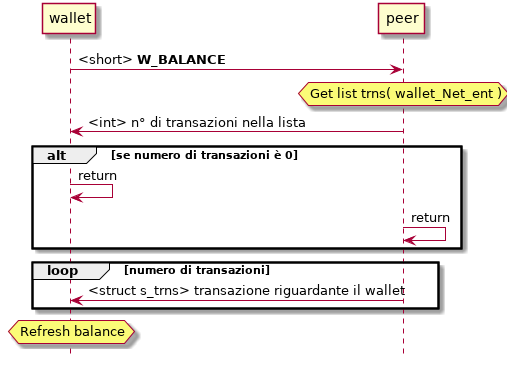
\includegraphics[scale=0.40]{w_balance.png}    
  \caption{richiesta di saldo}
  \label{fig:w_balance}
\end{figure}


